\chapter{Herramientas utilizadas para el laboratorio} \label{chap:herramientas}
Para el desarrollo de éste laboratorio, hicimos uso de herramientas de desarrollo, en su mayoría, basadas para entornos Linux, ya que, he percatado de que tiene mejor rendimiento y mejores resultados que trabajar dentro del sistema operativo Windows.

\section{Entorno de desarrollo}
Se usaron las siguientes herramientas.

\begin{itemize}
\item WSL para Windows.
\item Python 3.
\item freegut-dev.
\item Neovm
\item Anaconda
\end{itemize}

\section{Organización del proyecto.}
\subsection{Librerías utilizadas.}
Como se mencionó en la anterior lista, he decidido presindir del lenguaje de programación Python para el desarrollo del laboratorio. Puesto que es un lenguaje en la que me he desempeñado en trabajar desde hace un buen tiempo desde que estudio en la universidad.

\begin{figure}[H]
\centering
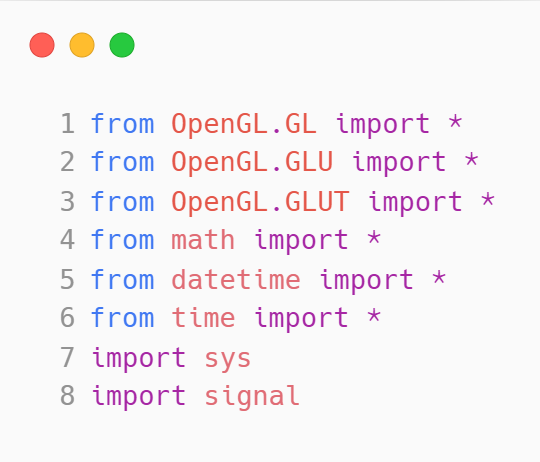
\includegraphics[width=0.4\textwidth]{../img/chapter01/1.png}
\caption{Librerías usadas para el laboratorio}
\label{fig:librerias_py}
\end{figure}

Las librerías más importantes para el laboratorio son las que vienen con PyOpenGL, que vienen con sus clases \textbf{GL, GLU y GLUT}, las cuales ejecutan las funciones y comamdos de OpenGL en Python.

En segundo lugar, tenemos la librería de \textbf{Time y Datatime} para el manejo del tiempo y de las fechas, nos ayuda a saber como está la hora y como ésta va repercutiéndose en el reloj.

Otra librería que no tiene mucho que ver con el uso de OpenGL, pero que, hace que sea más estilizado el programa, es la librería sys que, llama comandos de la terminal, como por ejemplo, limpiar la consola, realizar o llamar comandos, entre otras acciones que hacemos dentro de la terminal, y que en Python nos ayuda a ejecutar dentro del programa.

\subsection{Árbol del proyecto.} \label{subsec:arbol}
El archivo en general cuenta con una clase main que es la principal, contamos con una carpeta llamada \textbf{components}, en donde están los archivos \textbf{clock, display y draw}, la primera, es la clase en donde está trabajada las funciones que tienen que ver con la organización del reloj, la clase display, es la clase en donde se encuentra el método para la iniciación de la ventana, que es la gui en donde se visualiza el reloj, por último, está la clase draw, en donde están los métodos en donde se hace la manipulación de los elementos del reloj.

\begin{figure}[H]
	\centering
	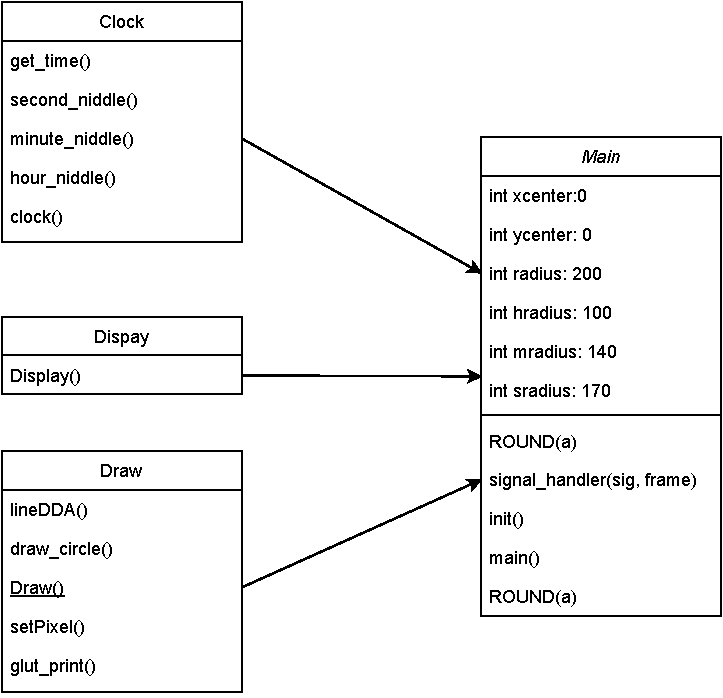
\includegraphics[width=0.8\textwidth]{../img/chapter02/3.pdf}
	\caption{Diagrama de clases del proyecto.}
	\label{fig:diagrama_clases}
\end{figure}







